%%-*-latex-*-

\documentclass[wide]{slides}

% Language
%
\usepackage{hyphenat}          % \hyp{} is a breakable dash
\usepackage{alltt}

\frenchspacing  % Follow French conventions after a period

% Maths & Logic
%
\usepackage{stmaryrd}
\usepackage{mathpartir}

% Graphics
%
\usepackage{graphicx}

% New environments and commands
%

% Input files
%
../TeX/commands.tex

% ----------------------------------------------------------------
% Document
%
\maintitle{Formal Methods in Software Engineering}
\mainauthor{\textbf{Christian Rinderknecht}\\
  {\small\url{Christian.Rinderknecht@tezcore.com}}\\
\Nomadic}
\confname{Tezos Masterclass}
\confshortname{Tezos}
\confdate{19 October 2018}

\begin{document}

\maketitle

\begin{slide}
  \title{Organisation and contributions}

  \begin{center}
    \textbf{Caleb Kow}\\
    \textbf{Diego Olivier Fern\'andez Pons}\\
    \textit{Tezos SouthEast Asia}\\
    Singapore
  \end{center}

\end{slide}

\begin{slide}
  \title{A personal introduction}

  \begin{itemize}

    \item My alma mater is \emph{Universit\'e Pierre et Marie Curie}
      (UPMC, a.k.a. Paris~6).

    \item I did my doctoral studies at \Inria, one of the most
      prestigious research institutes in informatics in France.

    \item I was a member of the team that developed the programming
      language \OCaml.

    \item I went on to work as an engineer, a researcher and a
      professor for many years, across several countries (France,
      Korea, Hungary, Sweden), both in academia and private
      industries.

    \item I recently joined the core development team behind the
      \Tezos blockchain, where I will be caring for compiler
      construction and domain\hyp{}specific languages.

  \end{itemize}

\end{slide}


\begin{slide}
  \title{A personal introduction}

  \begin{minipage}{0.5\linewidth}
    I have written a book about functional programming.
  \end{minipage}%
  \begin{minipage}{0.5\linewidth}
    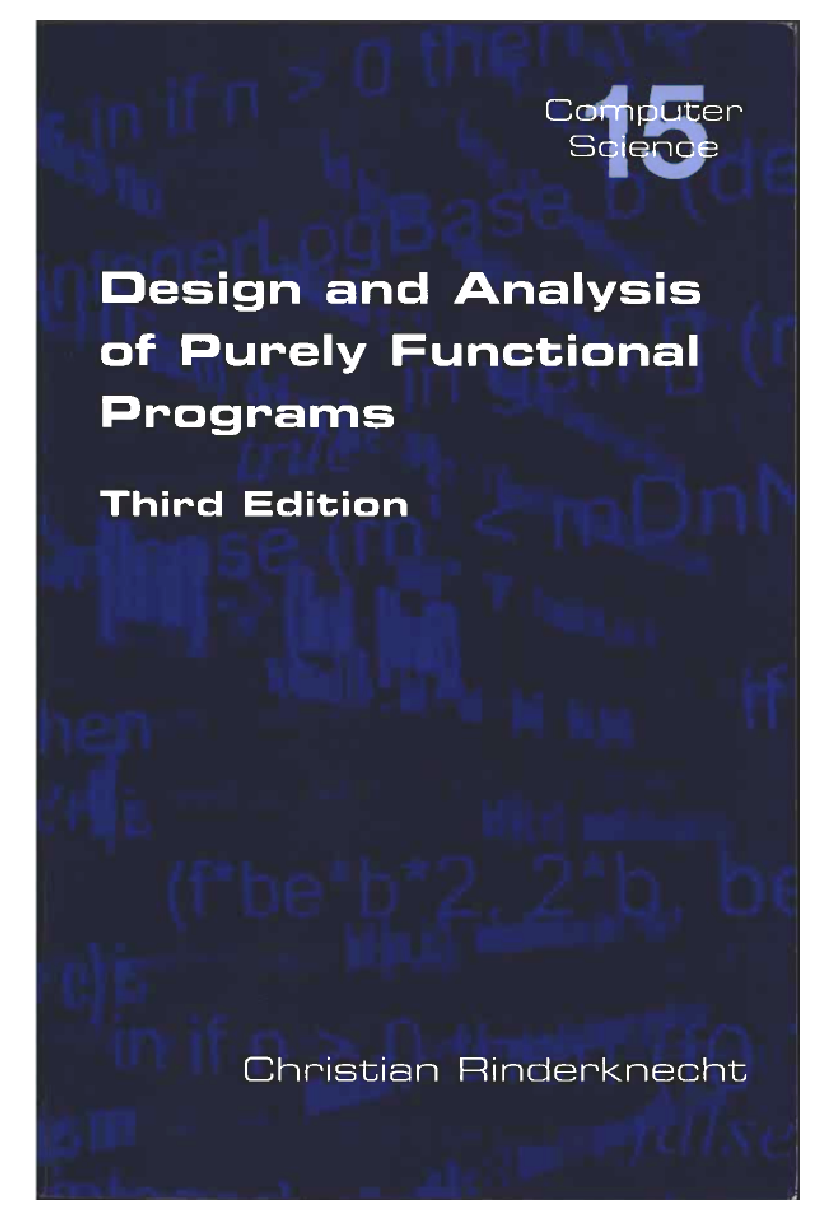
\includegraphics[scale=0.35]{my_book.eps}
  \end{minipage}%

\end{slide}

\begin{slide}
  \title{Introduction}

  \begin{itemize}

    \item This lecture is meant to present what \textbf{formal
      methods} are, in particular in the context of \textbf{software
      engineering}.

    \item It provides you with the industrial context and theoretical
      framework within which you can proceed to practical knowledge.

    \item Some of these formal methods and tools are used by \Tezos,
      or may be used.

    \item For instance, I will teach you a bit of \OCaml, which is
      used for all the code base of the \Tezos blockchain.

    \item This is the first of a series of lectures which hope to
      entice you to think how to contribute academic research or to
      become a successful engineer in leading or emerging industries
      (transport, aerospace, smart cards and... \textbf{blockchain}!).

  \end{itemize}
\end{slide}

\begin{slide}
  \title{Complex software is everywhere... and has bugs}

  \begin{center}
    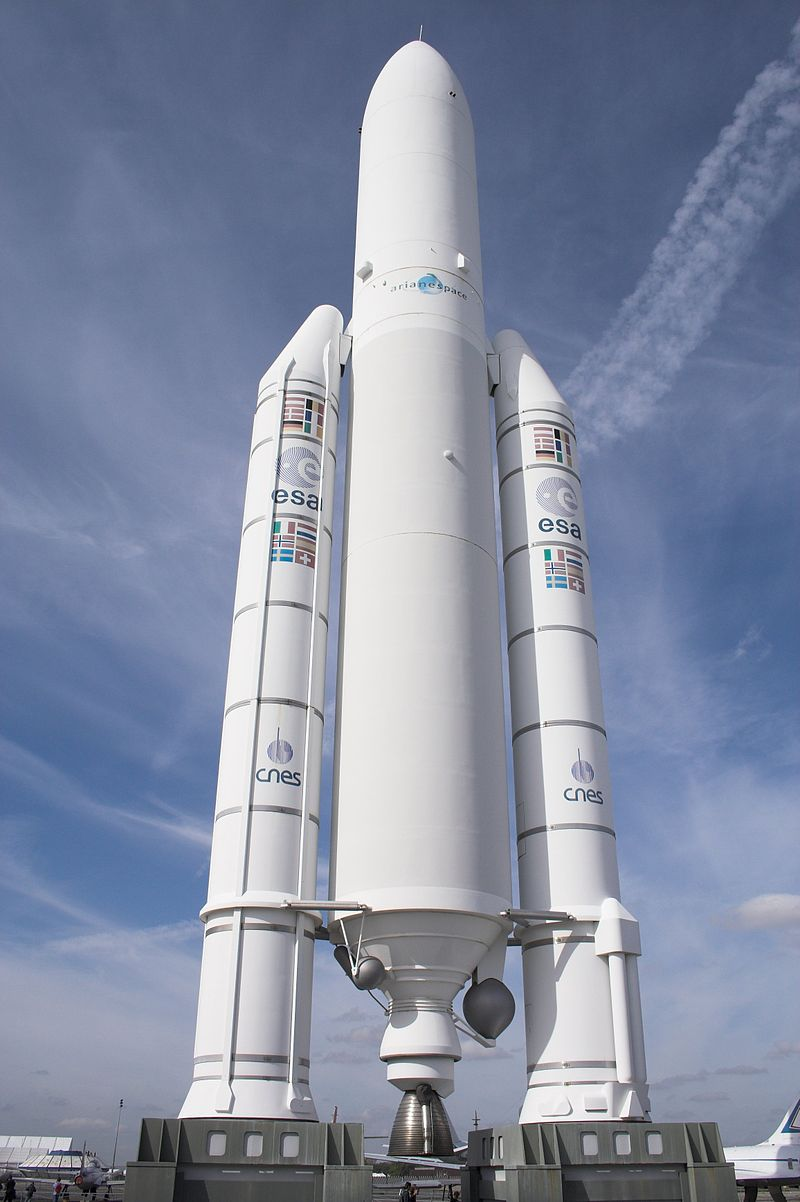
\includegraphics[scale=0.6]{Ariane_5.eps}
  \end{center}

  \centerline{Ariane 5. Credit: ignis, GFDL, CC BY-SA-2.5,2.0,1.0.}

\end{slide}

\begin{slide}
  \title{The case of Ariane~5}

  \begin{itemize}

    \item In June 1996, the maiden launch of the European rocket
      Ariane~5 ended in its self\hyp{}destruction.

    \item The cause was in the software controlling the trajectory.

    \item This piece of software was designed with the requirements of
      Ariane~4, \textbf{not} Ariane~5.

    \item Accordingly, some ranges of physical parameters were taken
      from Ariane~4, and wrongly assumed in the programming of
      Ariane~5.

    \item Therefore, certain errors were deemed impossible for
      physical reasons and not handled in the code.

    \item During the flight, a value overflowed, causing an exception
      to be raised, but not handled, which lead to the
      self\hyp{}destruction of the launcher (the control system
      believed that the rocket was off\hyp{}course).

  \end{itemize}

\end{slide}

\begin{slide}
  \title{The case of Ariane~5}

  \begin{itemize}

    \item The language used to program that piece of software in
      Ariane~5 was \Ada.

    \item \Ada is a programming language originally designed in France
      in the early 80s, before it became the official language for
      most developments for the defence of the USA.

    \item \Ada is used a lot in critical embedded systems, deployed in
      transport, aerospace and defence.

    \item The language was carefully designed so it lends itself well
      to all sorts of \textbf{static analyses}.

    \item These analyses are static because they are performed by the
      \Ada compiler itself, or by other tools that read the source
      code.

    \item Their aim can vary, but perhaps the most important is
      \textbf{the detection of run\hyp{}time errors} before the code
      is deployed.

  \end{itemize}

\end{slide}

\begin{slide}
  \title{The case of Ariane~5 / The after...math}

  \begin{itemize}

    \item The catastrophic failure of the first Ariane~5 incurred a
      very high cost, and the loss of ten years of research and
      development in satellite technology.

    \item \Ada itself is not to blame.

    \item Instead of going into the details of what went wrong, let us
      consider what happened next.

    \item Some researchers at \Inria (Gonthier \& Deutsch) proposed a
      static analyser for \Ada that could have caught the error that
      lead to the loss of Ariane~5, and discovered many other errors.

    \item The mathematical theory they used to analyse the software is
      called \textbf{abstract interpretation}.

    \item This powerful theory was invented in the 70s by the French
      researchers Patrick and Radhia Cousot.

  \end{itemize}
\end{slide}

\begin{slide}
  \title{PolySpace Technologies}

  \begin{itemize}

    \item In 1999, a start-up company called \textbf{PolySpace
      Technologies} was founded in France by Alain Deutsch (\Inria)
      and Daniel Pilaud (co\hyp{}inventor of \Lustre, a declarative
      language for programming synchronous systems).

    \item I joined that company in 2000 to work on the static analysis
      of JavaCard.

    \item The idea was to translate JavaCard and other languages
      (\Clang and \Cpp) to \Ada, for which there was already a static
      analyser, following the explosion of Ariane~5.

    \item The translation did not need to preserve all behaviours,
      only those who could go wrong (run\hyp{}time errors).

    \item The company was a success and is now part of
      \textbf{Mathworks Inc.}, known for MATLAB and \Simulink.

    \item PolySpace (the tool) is well known in the avionics industry.

  \end{itemize}

\end{slide}

\begin{slide}
  \title{Abstract interpretation}

  \begin{itemize}

    \item \textbf{Abstract interpretation} is a general framework to
      analyse programs and systems.

    \item It makes an \textbf{over\hyp{}approximation} of the
      behaviours of a program, then deduce properties on those, and
      finally translates back the abstract properties in terms of the
      original behaviours of the program.

    \item Abstract interpretation is used to replace a system with a
      possibly infinite or very large number of states with a system
      that has a small number of states that can all be checked
      exhaustively.

  \end{itemize}

\end{slide}

\begin{slide}
  \title{Abstract interpretation}

  \begin{itemize}

    \item For example, let us consider a simple program in \OCaml, a
      functional language, that prints a message depending on the sign
      of the square of its input:
\begin{alltt}

\textbf{let} f (p) =
  \textbf{let} p2 = p * p \textbf{in}
  \textbf{if} p2 < 0 \textbf{then} Printf.printf "Negative"
  \textbf{else} \textbf{if} p2 > 0 \textbf{then} Printf.printf "Positive"
        \textbf{else} Printf.printf "Zero"

\end{alltt}

    \item We aim to answer the question:
      \begin{quote}
        \textit{Are there inputs for which a run of this program would
          print ``\texttt{Negative}''?}
      \end{quote}

  \end{itemize}

\end{slide}

\begin{slide}
  \title{Abstract interpretation}

  \begin{itemize}

    \item If we identify the \OCaml operator ``\texttt{*}'' with the
      mathematical addition ``\(\times\)'', then the answer is
      obvious: \textbf{no}.

    \item But ``\texttt{*}'' is not ``\(\times\)'', simply because
      ``\texttt{p}'' is not an element of~\(\mathbb{N}\).

    \item \OCaml integers are those of the underlying hardware
      architecture. The number ``\texttt{p}'' is encoded as a
      \textbf{\(2\)-complement binary number}.

    \item The idea consists in interpreting the leftmost bit as a
      negative positional value, that is to say
      \begin{equation*}
        p = (b_{n-1}b_{n-2}\dots{b_0})_2
      \end{equation*}
      means
      \begin{equation*}
        p = -b_{n-1} \times 2^{n-1} + b_{n-2} \times 2^{n-2} + \dots + b_0
      \end{equation*}
      Thus, in an \(8\)-bit \(2\)-complement binary number, the
      leftmost bit has a positional value of \(-128\) rather than
      \(+128\). For example, \(p = (11110101)_2\) is interpreted as
      \begin{equation*}
        \begin{array}{rrrrrrrr}
          -128 & \mathbf{64} & \mathbf{32} & \mathbf{16} & 8 &
          \mathbf{4} & 2 & \mathbf{1}\\
          \hline
          1 &  1 &  1 &  1 & 0 & 1 & 0 & 1
        \end{array}
        \end{equation*}
      \begin{equation*}
        -128 + 64 + 32 + 16 + 4 + 1 = -11
      \end{equation*}

  \end{itemize}

\end{slide}

\begin{slide}
  \title{Abstract interpretation}

  \begin{itemize}

    \item It is easy to test the sign of such a number: if the
      leftmost bit is~\(1\), the number is negative; if it is~\(0\),
      then the number is positive or zero. That is because the
      greatest number with the leftmost bit set to~\(1\) is
      \((11...1)_2 = -2^{n-1} + (2^{n-2} + 2^{n-3} + \dots + 2^0) =
      -2^{n-1} + (2^{n-1} - 1) = -1 < 0\).

    \item \emph{A number is negative if, and only if, its leftmost bit
      is~\(1\).}

    \item But the algorithm for multiplying two \(2\)-complement
      binary numbers is not straightforward.

    \item It is not possible in practice to try all machine integers
      to test that program on a 64-bit architecture. (That would be
      \(2^{64} = 18,446,744,073,709,551,616\) numbers.)

  \end{itemize}

\end{slide}

\begin{slide}
  \title{Abstract interpretation}

  \begin{itemize}

    \item Let us imagine now that we abstract \OCaml integers to only
      keep track of their sign: we have only \emph{three} abstract
      values for each number now.
      \begin{alltt}

\textbf{type} abstract\_int = Positive | Negative | Zero
      \end{alltt}

    \item The multiplication can be abstracted accordingly:
      \medskip
\begin{alltt}
\textbf{let} abstract\_mult = \textbf{function}
  Negative, Negative \(\rightarrow\) Positive
| Negative, Positive \(\rightarrow\) Negative
| Positive, Negative \(\rightarrow\) Negative
| Positive, Positive \(\rightarrow\) Positive
|          _,      Zero \(\rightarrow\) Zero
|      Zero,          _ \(\rightarrow\) Zero

\end{alltt}

  \end{itemize}

\end{slide}


\begin{slide}
  \title{Abstract interpretation (continued)}

  \begin{itemize}

      \item The original program is also abstracted:
\begin{alltt}

\textbf{let} abstract\_f (p) =
  \textbf{let} p2 = abstract\_mult (p,p) \textbf{in}
  \textbf{if} p2 = Negative \textbf{then} Printf.printf "Negative"
  \textbf{else} \textbf{if} p2 = Positive \textbf{then} Printf.printf "Positive"
        \textbf{else} Printf.printf "Zero"

\end{alltt}

    \item The \textbf{correctness} of the abstraction is expressed as:
      \begin{alltt}

abstract (f (x)) = abstract\_f (abstract x)

      \end{alltt}

  \end{itemize}

\end{slide}

\begin{slide}
  \title{Abstract interpretation / An illustration}

  \begin{itemize}

    \item The abstract program can now be tested on three abstract
      values:
\begin{alltt}
abstract\_f (Negative) = Positive
abstract\_f (Zero)      = Zero
abstract\_f (Positive) = Positive
\end{alltt}

    \item Therefore, the abstract program can never print
      ``\texttt{Negative}'', and neither can the original.

    \item This example showcases the use of abstract interpretation to
      find \textbf{dead code}, that is, impossible runs of a program.

  \end{itemize}

\end{slide}

\begin{slide}
  \title{Abstract interpretation / An illustration}

  \begin{itemize}

    \item Abstract interpretation can also be used to \textbf{prove
      the absence of errors}, or to find errors.

    \item As an illustration, let us consider a system whose states
      are pairs of positive natural numbers, represented as
      coordinates on a quarter of plane.

    \item A \textbf{state} is all the information characterising a
      system running at a given point in time (memory contents,
      program counter, files, network buffers, etc.)

    \item Some states are coloured in \textcolor{red}{red} to denote
      that they are erroneous: this is the property ``To be
      erroneous.''

    \item A behaviour of a system, or \textbf{trace}, can be thought
      as a line from one state to the next. We show four traces as
      black, thick lines.

    \item One of the traces actually ends in an error.

  \end{itemize}

\end{slide}

\begin{slide}
  \title{Abstract interpretation / An illustration}

  \begin{center}
    \includegraphics[bb=95 428 500 727, scale=0.64]{traces.eps}
  \end{center}

\end{slide}

\begin{slide}
  \title{Abstract interpretation / An illustration}

  \begin{itemize}

    \item We need to characterise the erroneous states in a simple
      manner, at the cost of over\hyp{}approximating them: this means
      to abstract the property ``To be erroneous'' so it becomes
      easier to check.

    \item For example, we can abstract the error property by a red
      square containing the set of erroneous states, instead of being
      the set itself.

    \item A square can be defined by three numbers only, and it is
      easy to check whether a given state belongs to it: if so, we
      deem it an error.

    \item In our example, this creates \textbf{false positives}, that
      is, states inside the square that are not actual errors.

  \end{itemize}
\end{slide}

\begin{slide}
  \title{Abstract interpretation / An illustration}

  \begin{center}
    \includegraphics[bb=95 428 500 727, scale=0.64]{traces.eps}
  \end{center}

\end{slide}

\begin{slide}
  \title{Abstract interpretation / An illustration}

  \begin{center}
    \includegraphics[bb=95 428 500 727, scale=0.64]{traces_square.eps}
  \end{center}

\end{slide}

\begin{slide}
  \title{Abstract interpretation / An illustration}

  \begin{center}
\includegraphics[bb=95 428 500 727,scale=0.64]{traces_square_cropped.eps}
  \end{center}

\end{slide}

\begin{slide}
  \title{Abstract interpretation / An illustration}

  \begin{itemize}

    \item To reduce the number of false positives, we \textbf{refine
      the abstract property} so it fits better the erroneous states.

    \item For instance, we could use another polygon to cover more
      tightly the erroneous states.

    \item Let us try an hexagon: to define it, we need the same amount
      of information as for a square, but the inclusion property is
      slightly more complex.

    \item This is better, but one trace remains a false positive.

    \item In general, false positives are inevitable if the property
      is complex enough, so trade\hyp{}offs are necessary.

  \end{itemize}

\end{slide}

\begin{slide}
  \title{Abstract interpretation}

  \begin{center}
    \includegraphics[bb=85 428 500 727, scale=0.64]{traces_square_cropped.eps}
  \end{center}

\end{slide}

\begin{slide}
  \title{Abstract interpretation}

  \begin{center}
    \includegraphics[bb=85 428 500 727, scale=0.64]{traces_hexagon.eps}
  \end{center}

\end{slide}

\begin{slide}
  \title{A success story: the Parisian m\'etro line~14}

  \begin{center}
    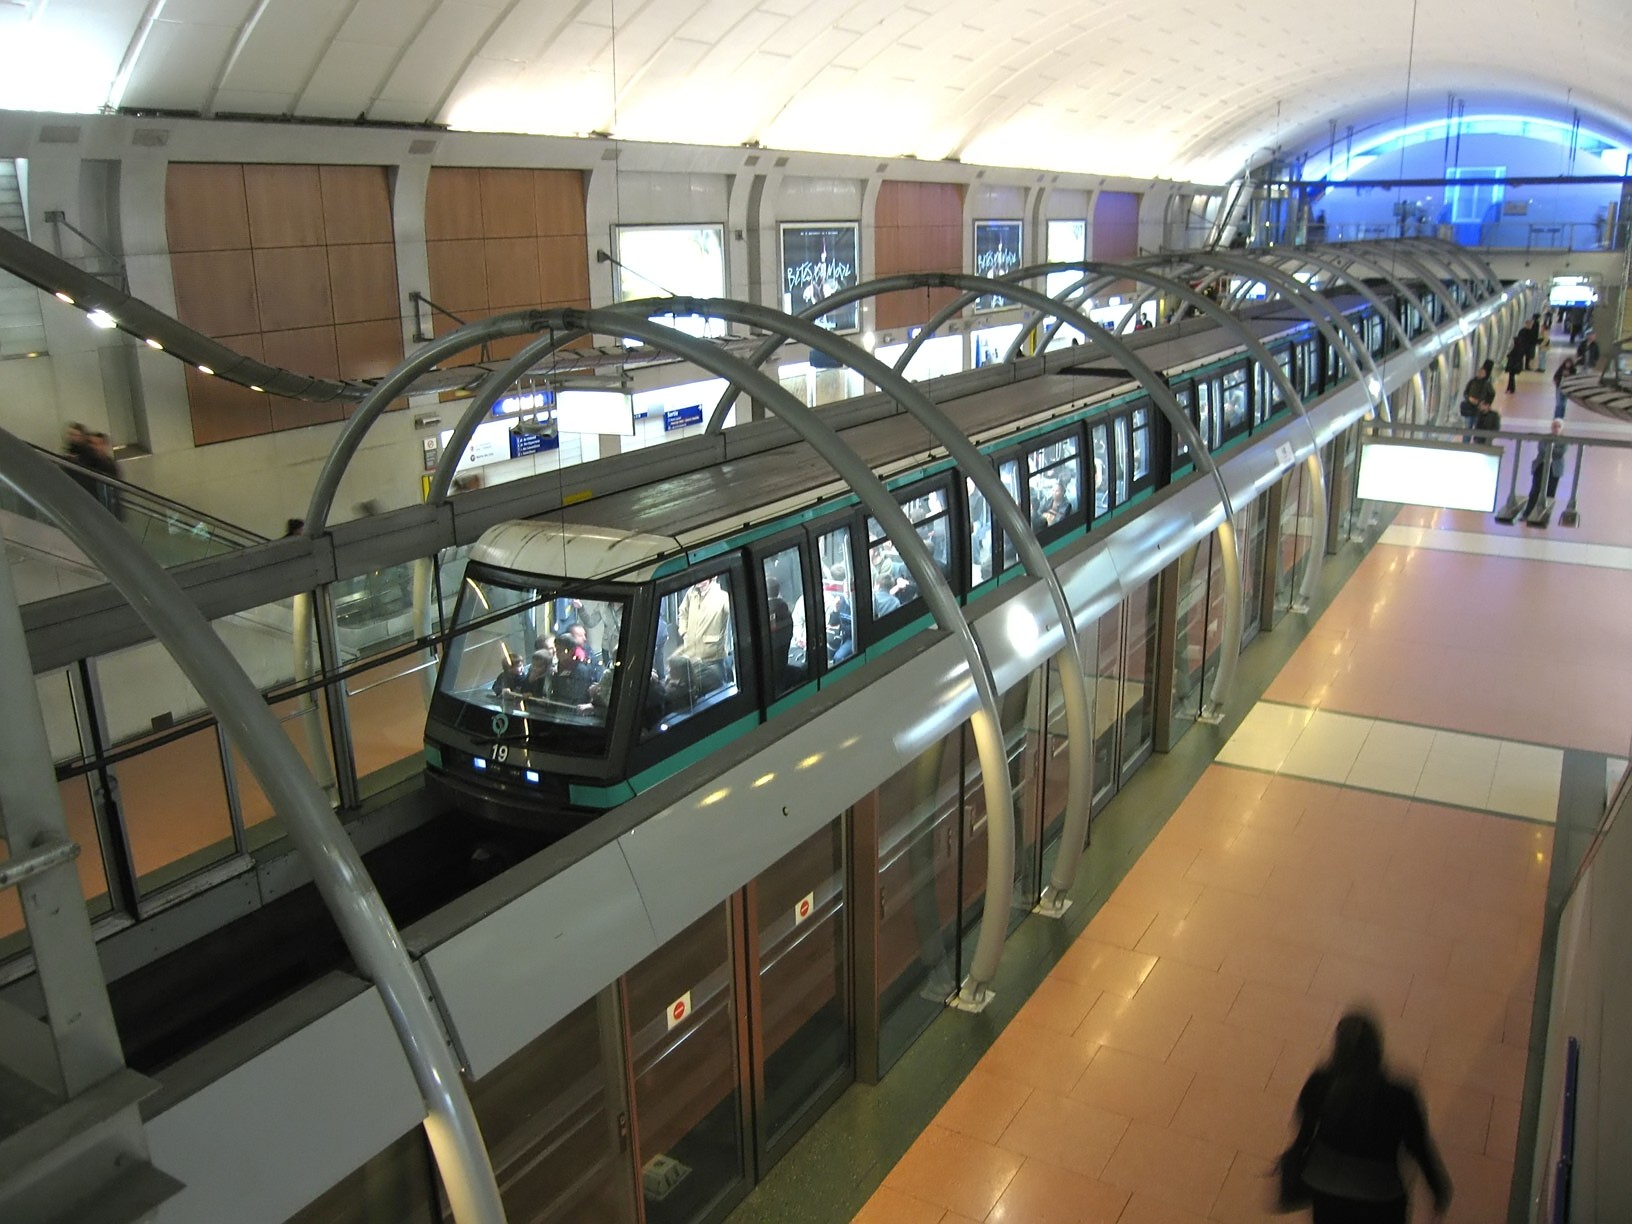
\includegraphics[scale=0.6]{ligne-14-Chatelet.eps}
  \end{center}

  \centerline{M\'etro line~14. Credit: Pline, CC BY-SA-3.0}

\end{slide}

\begin{slide}
  \title{The Parisian m\'etro line~14}

  \begin{itemize}

    \item In October 1999, opened in Paris the first entirely
      automated metro line (number~14).

    \item Some people thought that the trains were controlled at a
      distance, but they actually moved and stopped based on decisions
      taken by themselves, with inputs from sensors and communication
      networks.

    \item To ensure such a high\hyp{}level of safety and continuity of
      service, the company Matra Transport used formal methods from
      the start of the project.

    \item After the success of that new metro line, an existing metro
      line (number 1) has been automatised successfully.

    \item \textbf{Railways signalling systems} are a major user of
      formal methods, due to the high safety requirements.

  \end{itemize}
\end{slide}

\begin{slide}
  \title{The Parisian m\'etro line~14}

  \begin{itemize}

    \item The train system comprises four subsystems:
      \begin{enumerate}

        \item the automatic pilot and signalling system,

        \item the operation control centre,

        \item the platform doors,

        \item the audio-video system.

      \end{enumerate}

    \item Only the first subsystem includes software that is critical
      to the safety of the passengers.

    \item It controls the movement of trains (speed, traction power,
      routes) and the doors (on\hyp{}board and on the platforms).

    \item It sends any alarm to the operation control centre.

  \end{itemize}

\end{slide}

\begin{slide}
  \title{The Parisian m\'etro line~14}

  \begin{itemize}

    \item The system architecture is naturally distributed and
      is made of
      \begin{enumerate}

        \item the line equipment, in the operation control centre,

        \item the wayside equipment along the tracks,

        \item the on\hyp{}board equipment.

      \end{enumerate}

    \item They are interlinked via a high\hyp{}speed communication
      network.

  \end{itemize}

\end{slide}

\begin{slide}
  \title{The Parisian m\'etro line~14}

  \begin{itemize}

    \item In the operation control centre, operators monitor scheduled
      train programs for each day and supervise events received from
      the network.

      \item Platform doors prevent people from falling on the
        tracks. The train doors open only when they are aligned with
        the platform doors.

      \item If not properly aligned, there are emergency doors on the
        platform that can be manually opened.

      \item Audio and video feeds allows operators to monitor the
        inside the carriages and to speak with passengers (a
        high\hyp{}level of availability is required to ensure
        security).
  \end{itemize}

\end{slide}

\begin{slide}
  \title{The Parisian m\'etro line~14}

  \begin{itemize}

    \item In order to bring strong correctness assurances in software,
      it is paramount to carefully specify the expected behaviours and
      delimit the field of application of the mathematical proofs.

    \item The use of the \textbf{B~method} by Matra Transport
      International (now part of Siemens) for the Parisian metro
      line~14 is a case in point of this approach.

    \item Another example is the Calcutta metro, in 1992.

    \item The B~method was invented in the 80s by Jean-Raymond Abrial,
      a French researcher.

    \item It comprises
      \begin{enumerate}

        \item a formal notation to expression specifications,

        \item a design methodology,

        \item and software tools as a support.

      \end{enumerate}

  \end{itemize}

\end{slide}

\begin{slide}
  \title{The B~method}

  \begin{itemize}

    \item The formal \textbf{\Blang} is based on \textbf{set theory},
      which makes it very expressive.

    \item It enables the specification of a system and its expected
      properties into a model called an \textbf{abstract machine}.

    \item It also enables the proof of such properties (like safety):
      some as \textbf{system invariants} (properties that must hold on
      all states), some as \textbf{postconditions} to mathematical
      functions.

    \item A \textbf{proof assistant} then either automatically proves
      some of these theorems, or requests the engineer to prove them
      interactively.

    \item The B~method and its software tools allow the engineer to
      \textbf{refine} the abstract machine into a series of abstract
      machines until a \textbf{concrete machine} is obtained.

    \item A concrete machine is one that can be translated
      automatically into a programming language (\Clang or \Ada).

  \end{itemize}

\end{slide}

\begin{slide}
  \title{The B~method}

  \begin{itemize}

    \item Each abstract machine is, in turn, less and less
      \textbf{denotational}, and more and more \textbf{operational}.

    \item ``Operational'' means ``what a system does'', whereas
      ``denotational'' means ``what properties the system satisfies''.

    \item Step by step, the abstract machines become closer to
      \textbf{algorithms}, that is, functions operating over data
      structures, which is what a concrete machine is about.

    \item The other aspect of a concrete machine is that it is
      \textbf{deterministic}: there are no unspecified choices left in
      the control flow (``what to do next'' is always explicit).

  \end{itemize}

\end{slide}

\begin{slide}
  \title{The B~method / Refinement}

  \begin{center}
    \includegraphics[bb=71 350 385 721]{refinement.pdf}
  \end{center}

\end{slide}

\begin{slide}
  \title{The B~language / An abstract machine}

  \begin{itemize}

    \item An abstract machine in the B~language consists of
      \begin{itemize}

        \item \textbf{states}, that is, variables satisfying some
          invariant properties, and

        \item \textbf{operations}, that is, functions that change the
          state while maintaining the invariants, and return values.

      \end{itemize}

    \item The variables making up the state of an abstract machine can
      denote mathematical sets, relations, functions, etc.

    \item Operations are defined with
      \begin{itemize}

        \item \textbf{preconditions}: ``What is assumed about the
          state by the operation before starting'', and

        \item \textbf{postconditions}: ``What can be assumed about the
          state and return value after the operation is finished''.

      \end{itemize}

  \end{itemize}

\end{slide}

\begin{slide}
  \title{The B~language / An abstract machine}

  \begin{itemize}

    \item Let us specify in the B~language what is the Greatest Common
      Divisor (GCD) of two natural numbers.

    \item In English: ``The GCD of \(x\)~and~\(y\) is~\(d\) such that
      \(d\) divides both \(x\)~and~\(y\), and any divisor of~\(x\)
      and~\(y\) is lower than or equal to~\(d\).''

    \item In mathematical notation:
      \begin{equation*}
        \gcd(x,y) \mid x \quad\land\quad
        \gcd(x,y) \mid y \quad\wedge\quad
        \forall z.(z \mid x \;\;\wedge\;\; z \mid y
        \;\; \Rightarrow\;\; z \leqslant \gcd(x,y)).
      \end{equation*}

      \item The next slide shows the equivalent definition in the
        B~language (note that variables must be at least two
        characters long).
  \end{itemize}

\end{slide}

\begin{slide}
  \title{Greatest Common Divisor (abstract)}

\begin{alltt}
\textbf{MACHINE} gcd /* Greatest Common Divisor */
\textbf{OPERATIONS}
  rr <-- gcd (xx,yy) =
    \textbf{BEGIN}
      \textbf{PRE} xx : INT & 1 <= xx & xx < MAXINT
           yy : INT & 1 <= yy & yy < MAXINT
      \textbf{THEN}
        \textbf{ANY} dd \textbf{WHERE}
         dd : INT
            & (xx-(xx/dd)*dd = 0) & (yy-(yy/dd)*dd = 0)
            & !zz.(zz : INT & zz < MAXINT
                   & (xx-(xx/zz)*zz = 0)
                   & (yy-(yy/zz)*zz = 0) => zz <= dd)
        \textbf{THEN} rr := dd \textbf{END}
      \textbf{END}
    \textbf{END}
\end{alltt}

\end{slide}

\begin{slide}
  \title{The B~method / Refinement}

  \begin{itemize}

    \item The refinement from the initial abstract machine to the
      final concrete machine is stepwise and the engineer must provide
      more details about the low\hyp{}level aspects of the system,
      whilst proving the new specification is \textbf{correct and
        complete} with respect to the previous one (all its behaviours
      are expected by the previous one, and vice\hyp{}versa).

    \item This transitively entails that the concrete machine is
      \textbf{equivalent} to the initial abstract machine.

    \item The last step consists in the \textbf{generation of \Ada
      programs} which are thus, by construction, correct and complete
      with respect to the initial specification.

  \end{itemize}

\end{slide}

\begin{slide}
  \title{Greatest Common Divisor (concrete)}

\begin{alltt}
\textbf{REFINEMENT} gcd_R1 /* refinement of ... */
\textbf{REFINES} gcd /* the previous machine */
\textbf{OPERATIONS}
 rr <-- gcd (xx,yy) = /* No room to handle xx < yy */
   \textbf{BEGIN}
     \textbf{PRE} xx : INT & 1 <= xx & xx < MAXINT
          yy : INT & 1 <= yy & yy < MAXINT
     \textbf{VAR} rem, old_xx, old_yy \textbf{IN}
     \textbf{WHILE} (yy != 0)
       old_xx := x; old_yy := yy; rem := xx-(xx/yy)*yy;
       xx := old_yy; yy := rem;
     \textbf{INVARIANT} gcd (old_xx, old_yy) = gcd (old_yy, rem);
     \textbf{VARIANT} yy < old_yy; /* Termination */
     rr := xx;
   \textbf{END}
\end{alltt}

\end{slide}

\begin{slide}
  \title{The B~language / Ada}

  From the concrete machine, the following \Ada code fragment would be
  produced, were the tooling told to inline the values of the
  variables \texttt{rr}, \texttt{old\_xx} and \texttt{old\_yy}, which
  are only needed for logical reasons (to state the invariant and
  variant, and the final result), not computational ones.
\begin{alltt}
\textbf{function} GCD (Xx, Yy : Integer) \textbf{return} Integer \textbf{is}
  Rem : Integer;
  \textbf{while} Yy /= 0 \textbf{loop}
    Rem := Xx \textbf{mod} Yy;
    Xx := Yy;
    Yy := Rem;
  \textbf{end loop};
  \textbf{return} Xx;
\textbf{end} GCD
\end{alltt}

\end{slide}

\begin{slide}
  \title{Introduction (resumed)}

  \begin{itemize}

    \item Formal methods are methods and tools for software
      development that are grounded in theoretical computer science
      (informatics).

    \item Some expected benefits are:

      \begin{itemize}

        \item the reduction in maintenance costs (e.g., corrective
          maintenance),

        \item more robustness (by explicitly delineating the domain of
          validity) and, more generally,

        \item higher reliability and levels of confidence.

      \end{itemize}

    \item Formal methods are often applied in the making of
      \textbf{critical embedded systems} to guarantee safety and
      security, whenever human lives or large investments depend upon
      their correctness and continuity of service.

  \end{itemize}
\end{slide}

\begin{slide}
  \title{Astr\'ee}

  \begin{center}
    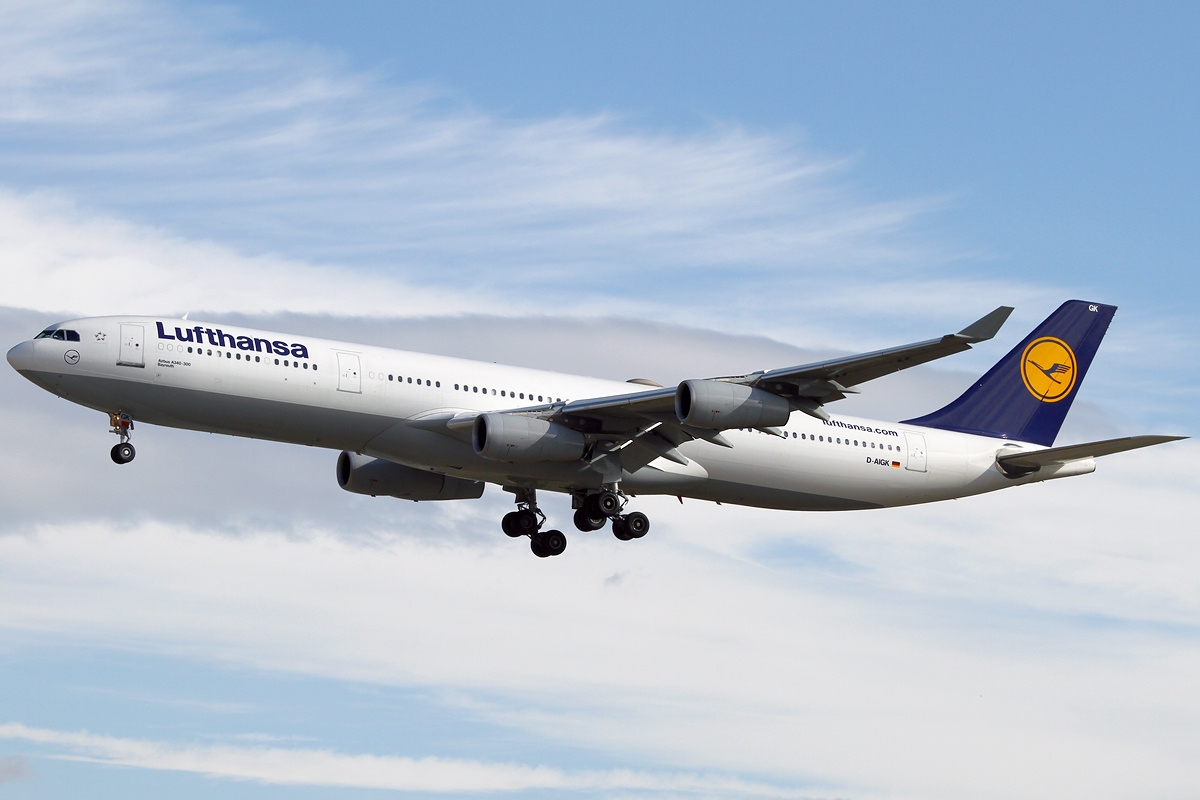
\includegraphics[scale=0.22]{Airbus_A340.eps}
  \end{center}

    \centerline{Airbus A340. Credit: Konstantin von Wedelstardt. GFDL
      1.2}

\end{slide}

\begin{slide}
  \title{The static analyser Astr\'ee}

  \begin{itemize}

    \item The usefulness of formal methods should not be
      underestimated. They have taken decades to mature from academic
      research to practical frameworks, and are becoming more and more
      widespread.

    \item Beyond PolySpace and the B~method, we can mention some other
      successful static analysers.

    \item \textbf{Astr\'ee} offers an abstract interpretation of
      \Clang programs to detect run\hyp{}time errors, in the same vein
      as PolySpace.

    \item It was designed at \'Ecole Normale Sup\'erieure (France) and
      is now commercialised by the German company AbsInt.

    \item In 2003, Astr\'ee proved automatically (on a standard PC)
      the absence of any run\hyp{}time errors in the primary flight
      control software of the Airbus A340 fly-by-wire system: 132,000
      lines of \Clang.

    \item Astr\'ee is written in \OCaml and PolySpace in
      \textsf{Standard ML}, the American cousin of \OCaml.

  \end{itemize}

\end{slide}

\begin{slide}
  \title{The static analyser Frama-C}

  \begin{center}
    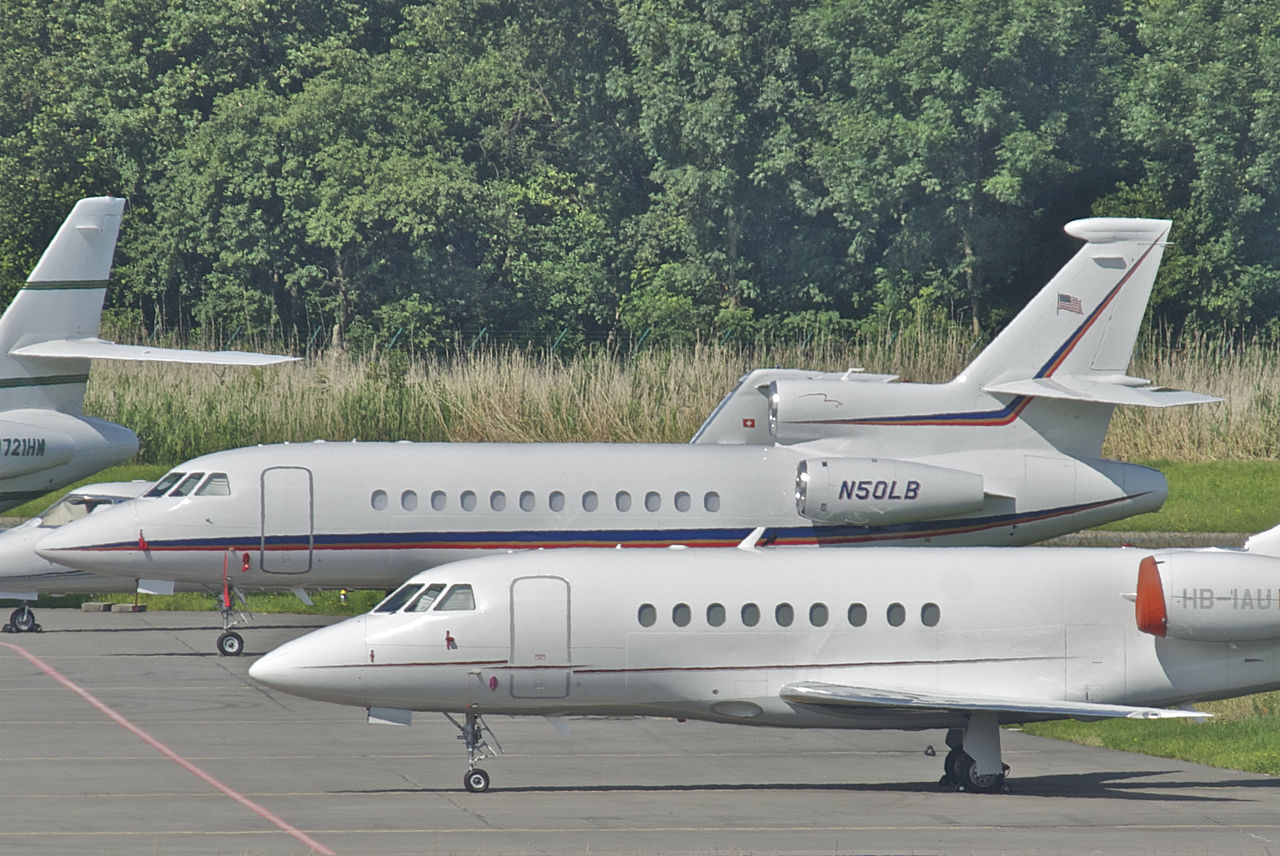
\includegraphics[scale=0.20]{Dassault_Falcon_900.eps}
  \end{center}

  \centerline{Dassault Falcon 900. Credit:  Aero Icarus, CC BY-SA-2.0}

\end{slide}

\begin{slide}
  \title{The static analyser Frama-C}

  \begin{itemize}

    \item Another well\hyp{}known static analyser for \Clang is
      \textbf{Frama-C}.

    \item It was designed by researchers at the CEA (France).

    \item Frama-C is actually a software suite which includes a static
      analyser, but also software to interactively prove that the
      source code satisfies some \textbf{functional specifications}
      provided by the user.

    \item Recently, Frama-C has been used by Dassault Aviation to
      detect common weaknesses in real\hyp{}time software running on
      the Falcon jets.

    \item In 2016, I joined the French company \textbf{TrustInSoft}
      that commercialises bespoke plug\hyp{}ins for Frama-C.

    \item The code base of Frama-C is almost entirely written in
      \OCaml (perhaps the largest \OCaml code base in the world).

  \end{itemize}

\end{slide}

\begin{slide}
  \title{Formal methods applied to compilers}

%  \hspace*{-30pt}
  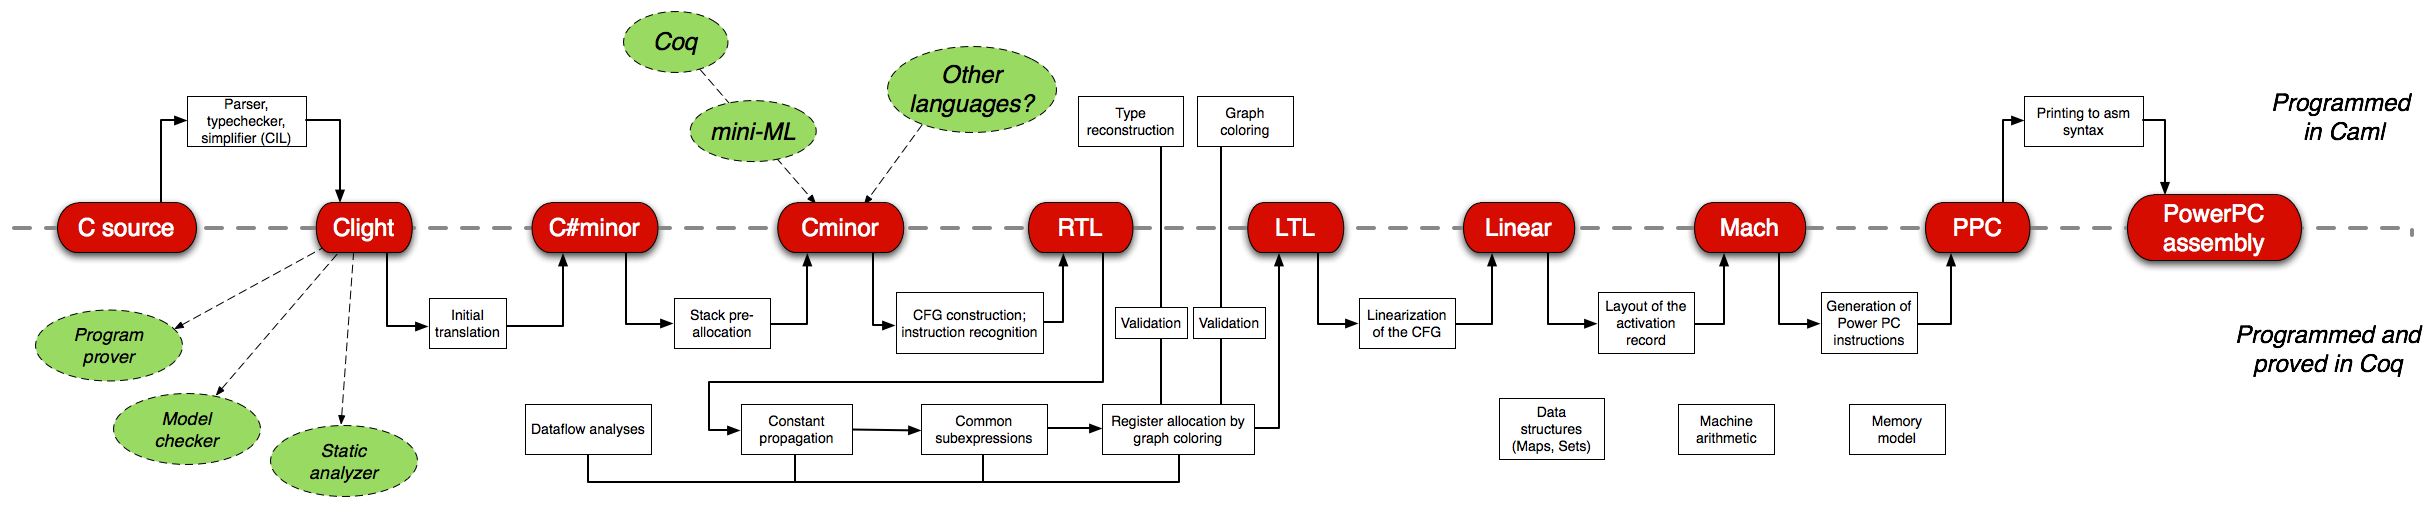
\includegraphics[scale=0.3,angle=0,origin=c]{CompCert_diagram.eps}

\end{slide}

\begin{slide}
  \title{Formal methods applied to compilers}

  \begin{itemize}

    \item Formal methods can also be applied to \textbf{compilers}.

    \item Compilers translate programs of high\hyp{}level languages
      (``close to human thought''), like \Clang, \Ada or \OCaml into
      programs of low\hyp{}level languages (``close to machine
      thought''), like assembly or byte\hyp{}code, and these two
      programs must be \textbf{operationally equivalent}.

    \item This means that all behaviours of the input program must be
      preserved in the output program (\textbf{completeness}) and all
      behaviours of the output must map to behaviours of the input
      (\textbf{soundness}, also called \emph{correctness}).

    \item Since \Clang is widespread in critical embedded software, it
      is desirable to consider \Clang compilers.

  \end{itemize}

\end{slide}

\begin{slide}
  \title{General architecture of a C compiler}

  The compiler is one link in a \textbf{tool chain}:
  \begin{center}
    \includegraphics[bb=71 350 405 721,scale=0.9]{compilation_chain.pdf}
  \end{center}

\end{slide}

\begin{slide}
  \title{General architecture of a C compiler}

  There are two phases to compilation: \textbf{analysis} and
  \textbf{synthesis}.
  \begin{enumerate}

    \item The analysis breaks up the source program into
      constituent pieces of an intermediary representation of the
      program.

    \item The synthesis constructs the target program from this
      intermediary representation.

  \end{enumerate}
  \begin{itemize}

    \item Actually, there can be many intermediary representations,
      each one getting closer to the target language.

    \item Each phase is itself decomposable into other phases,
      depending on the source and target languages.

  \end{itemize}

\end{slide}

\begin{slide}
  \title{General architecture of a C compiler}

  The first row makes up the analysis and the second is the synthesis.

  \begin{center}
    \includegraphics[scale=0.9, trim=0 5.8cm 2cm 0]{phases.pdf}
  \end{center}

  \begin{itemize}

    \item A real compiler has many more stages than shown above, and
      is always a complex piece of software where more errors are
      likely.

    \item Those errors can be silent: some erroneous code can be
      emitted only for certain classes of programs, which is a serious
      problem for embedded applications.

    \item Xavier Leroy at \Inria (France) has spearheaded the design
      and implementation of a \textbf{certified \Clang compiler},
      called \textbf{CompCert}, using \Coq.

  \end{itemize}

\end{slide}

\begin{slide}
  \title{A formally verified C compiler: CompCert}

  \begin{itemize}

    \item CompCert is certified because its \textbf{\OCaml code has
      been extracted from the specification} (of a large subset) of
      \Clang and intermediary representations, as well as from
      \textbf{semantic\hyp{}preserving transformations} between those
      representations, down to optimised assembly.

    \item John Regher and his colleagues are experts in finding bugs
      in \Clang compilers. They wrote, in 2011:
      \begin{quote}
        \textit{The striking thing about our CompCert results is that
          the middle\hyp{}end bugs we found in all other compilers are
          absent. [...] This is not for lack of trying: we have
          devoted about six CPU\hyp{}years to the task. The apparent
          unbreakability of CompCert supports a strong argument that
          developing compiler optimizations within a proof framework,
          where safety checks are explicit and machine-checked, has
          tangible benefits for compiler users.}
      \end{quote}
  \end{itemize}

\end{slide}

\begin{slide}
  \title{The proof assistant Coq}

   \begin{center}
     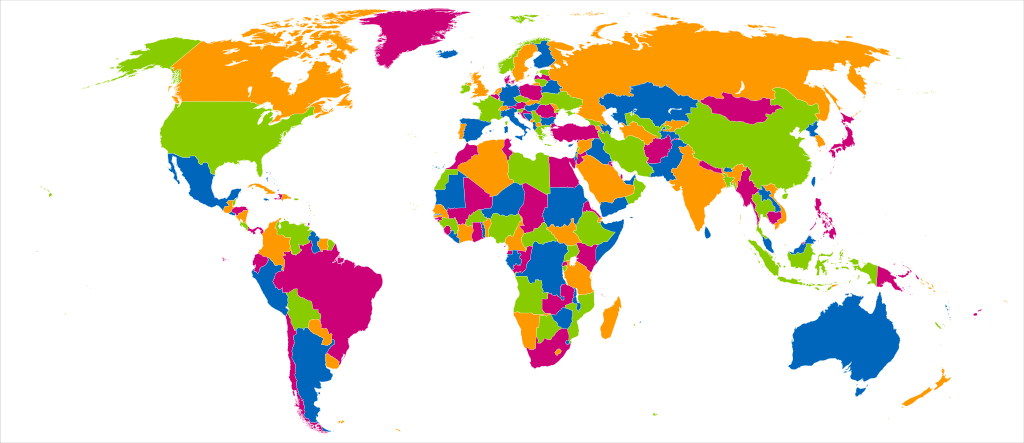
\includegraphics[scale=0.3]{world_map_with_four_colours.eps}
   \end{center}

   \centerline{Political map of the world. Credit: Fibonacci, CC BY-SA
     3.0}

\end{slide}

\begin{slide}
  \title{The proof assistant Coq}

  \begin{itemize}

    \item \Coq is a \textbf{proof assistant}, that is, a piece of
      software in which to express logical formulas, prove them and
      have the proofs checked automatically. It is an interactive
      tool, but it automates the search of some proof patterns
      (libraries called \textbf{tactics}).

    \item \Coq comes with a programming language named
      \textbf{Gallina} which is close to \OCaml, but \textbf{without
        side\hyp{}effects} and adding \textbf{dependent types}. This
      type system is more general than the type systems found in usual
      languages like \Java.

    \item \Coq features \textbf{code extraction}: it can generate an
      \OCaml program from the proof of its properties.

    %% \item A \textbf{constructive proof} is a proof in which for each
    %%   \(\exists\) quantifier, a witness is given: every object must be
    %%   explicitly built. In particular, this rules out the use of the
    %%   \textbf{law of excluded middle} of classical logic (\(\vdash A
    %%   \lor \neg A\)).

    \item Code extraction relies upon the \textbf{Curry\hyp{}Howard
      correspondence}, which states that a proof is analogous to a
      function, and the proved theorem is analogous to the type of
      that function.

    \item \Coq was created in 1989 by Huet and Coquand, at \Inria
      (France), where it is developed today. It is written in \OCaml.

  \end{itemize}

\end{slide}

\begin{slide}
  \title{Coq: Other Applications}

  Here is a list of compilers certified by \Coq:
  \begin{itemize}

    \item \textsf{CompCert}, an optimizing compiler for a subset of C
      by Xavier Leroy in 2012;

    \item \textsf{CertiCoq}, a compiler by researchers at Princeton,
      Edinburgh, Inria and Cornell in 2017;

    \item \textsf{Q*cert}, a query compiler by IBM Research in 2017;

    \item \textsf{Ergo}, a compiler from Ergo (a language of legal
      smart contracts) to \Michelson by Jerôme Siméon in 2018.

  \end{itemize}

   In graph theory, it was used to prove the \textbf{four colour
     theorem}, that states that countries in an arbitrary map can
   always be coloured with four colours (Gonthier, Microsoft Research,
   2008).

\end{slide}

\begin{slide}
  \title{Certified cryptographic primitives}

  \begin{center}
    
\includegraphics[scale=0.6]{heartbleed.eps}
  \end{center}

  \centerline{Heartbleed bug logo. Credit: Codenomicon, CC0 1.0}

\end{slide}

\begin{slide}
  \title{Certified cryptographic primitives / Heartbleed}

  \begin{itemize}

    \item In April 2014 was disclosed a bug in the OpenSSL
      cryptographic library introduced in 2012. The bug was named
      \textbf{Heartbleed} and given a logo to increase public
      awareness.

    \item The bug is due to improper input validation (missing bounds
      check) in the implementation of the TLS heartbeat extension and
      allows protected data to be read.  The bug allows stealing
      private keys and users' session cookies and passwords

    \item The faulty code was written by a PhD student at
      Fachhochschule Münster, and the OpenSSL core developer that
      reviewed the code did not notice the problem.

    \item Around 500,000 SSL certificates were compromised by the bug
      and had to be reissued.

    \item Canada Revenue Agency was stolen 900 social insurance
      numbers in 2014 due to the bug. The records of 4.5 million
      patients were accessed after a breach into the system of
      Community Health, a private hospital in the USA.

  \end{itemize}

\end{slide}

\begin{slide}
  \title{Certified cryptographic primitives / HACL*}

  Given how critical cryptographic primitives are, \Tezos uses
  \HACLstar, a formally verified cryptographic library, developed by
  the Prosecco team at Inria in collaboration with Microsoft
  Research.

  \begin{itemize}

    \item \HACLstar is written in \Fstar, an \textsf{ML}-style
      general-purpose functional programming language (with effects)
      aimed at program verification. \Fstar is a cousin of \OCaml and
      \Coq.

    \item The \Fstar code is then extracted into \Clang with the
      \textsf{KreMLin} tool.

    \item To generate \Clang code that is proven is correct, the
      \Fstar code is first transformed into \textsf{Low*}, a shallow
      embedding of a subset of \Clang into \Fstar with explicit memory
      management. The code is compiled from \textsf{Low*} to \Clang
      and compiled with a \Clang compiler (certified like CompCert, or
      not)

  \end{itemize}

\end{slide}

\begin{slide}
  \title{Certified cryptographic primitives / HACL*}

  According to the authors of \HACLstar,

  \bigskip

  \begin{quote}
    \textit{when compiled with GCC on 64-bit platforms, our primitives
      are as fast as the fastest pure C implementations in OpenSSL and
      Libsodium, significantly faster than the reference C code in
      TweetNaCl, and between 1.1\(\times\) and 5.7\(\times\) slower
      than the fastest hand-optimized vectorized assembly code [...]}
  \end{quote}

\end{slide}

\begin{slide}
  \title{F*}

  \begin{center}
    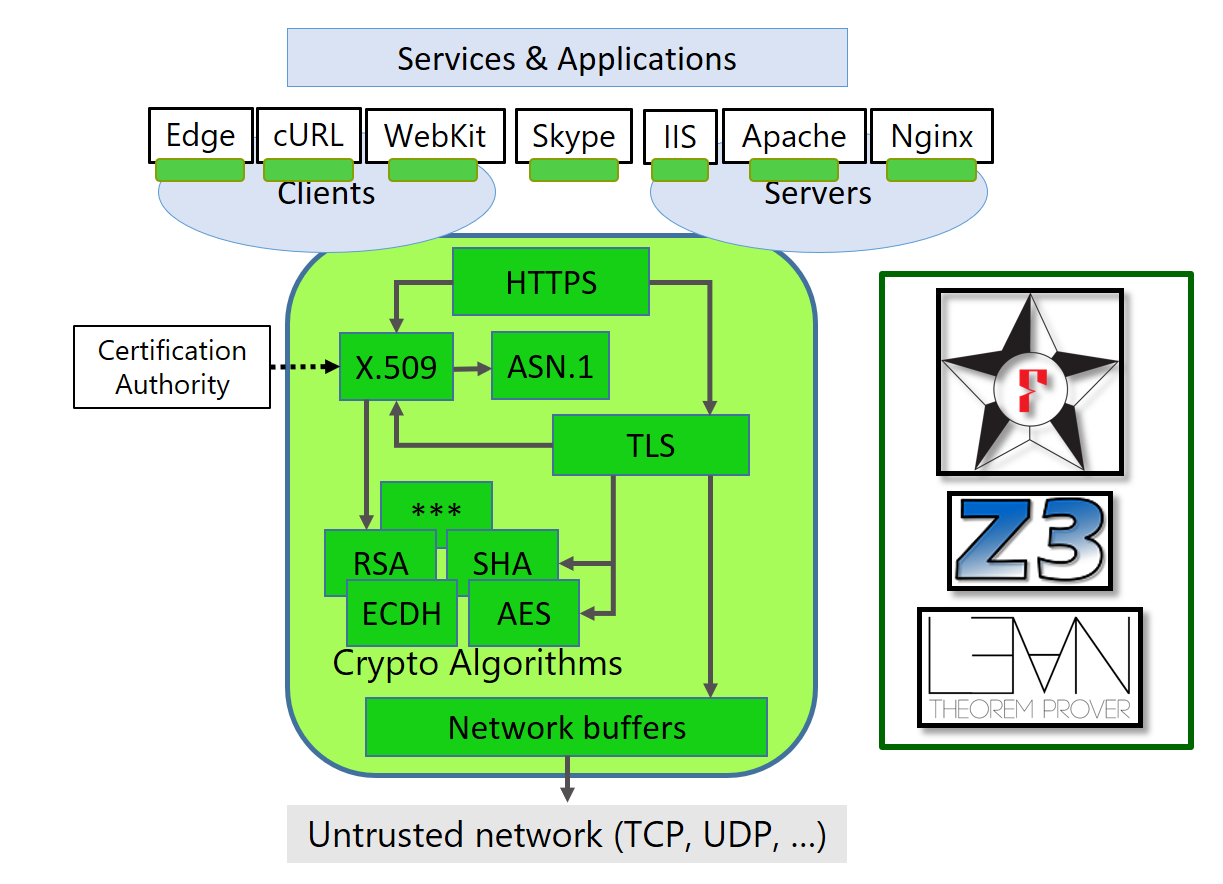
\includegraphics[scale=0.2]{SecureHTTPS.eps}
  \end{center}

\end{slide}

\begin{slide}
  \title{F*}

  \Fstar is an \textsf{ML}-style general-purpose functional
  programming language with effects aimed at program verification.

  \begin{itemize}

    \item It was designed and developed at the joint Microsoft
      Research-Inria Center.

    \item \Fstar programs can be extracted to efficient \OCaml,
      \Fsharp, or \Clang code.

    \item The \Fstar typechecker aims at proving that programs meet
      their specifications using a combination of \textbf{SMT solving}
      and interactive proofs.

    \item Like \Coq, \Fstar can also be helped with intermediate
      lemmas and tactics when it cannot prove automatically the
      properties of the code.

  \end{itemize}

  There is an online tutorial
  \url{https://www.fstar-lang.org/tutorial/}
\end{slide}

%% \begin{slide}
%%   \title{F*}

%%   \begin{center}
%%     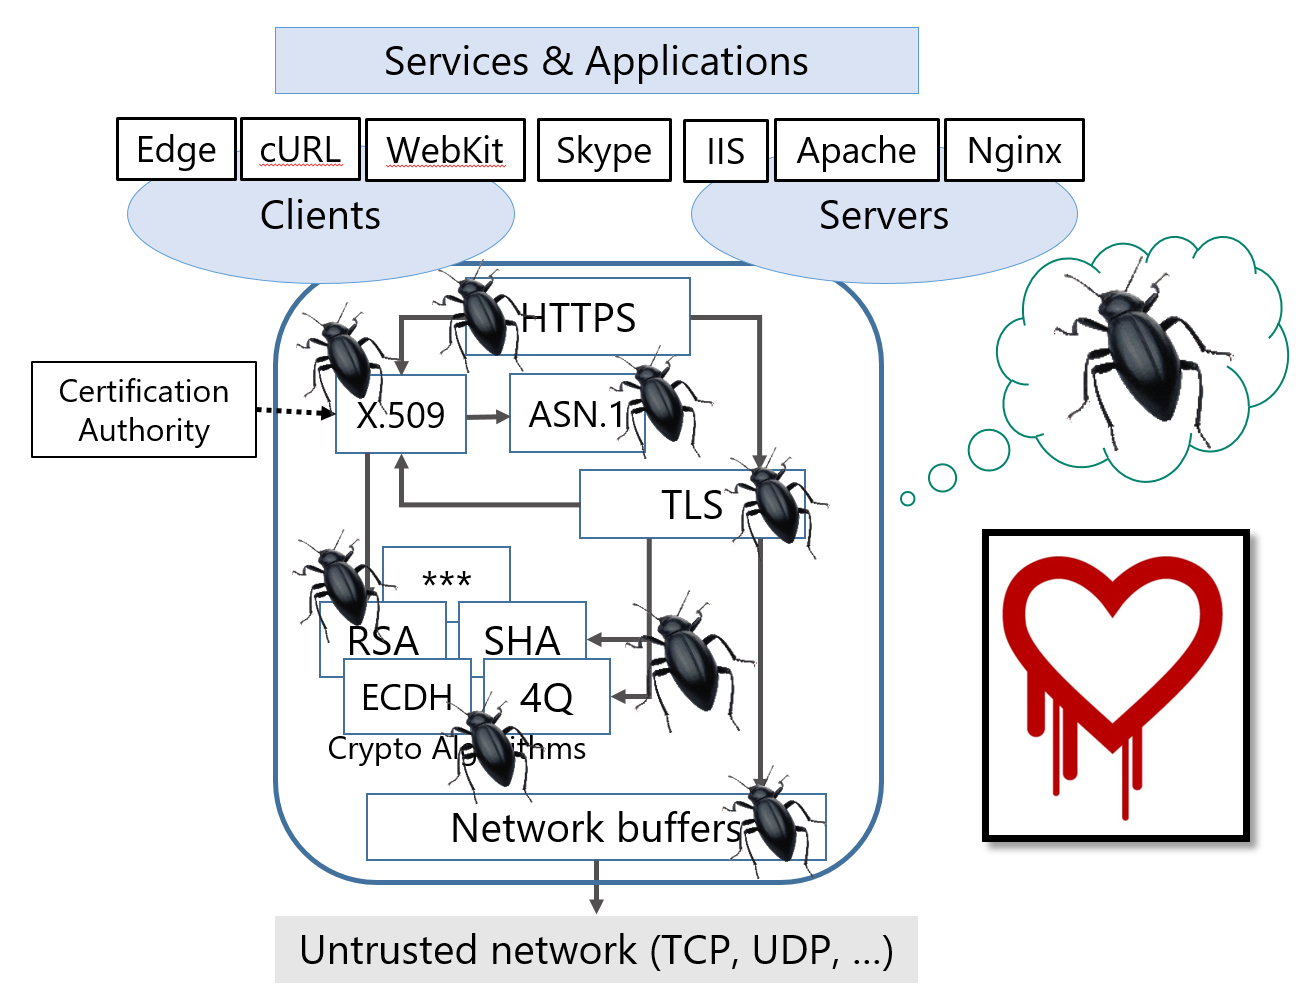
\includegraphics[scale=0.12]{InsecureHTTPS.eps}
%%     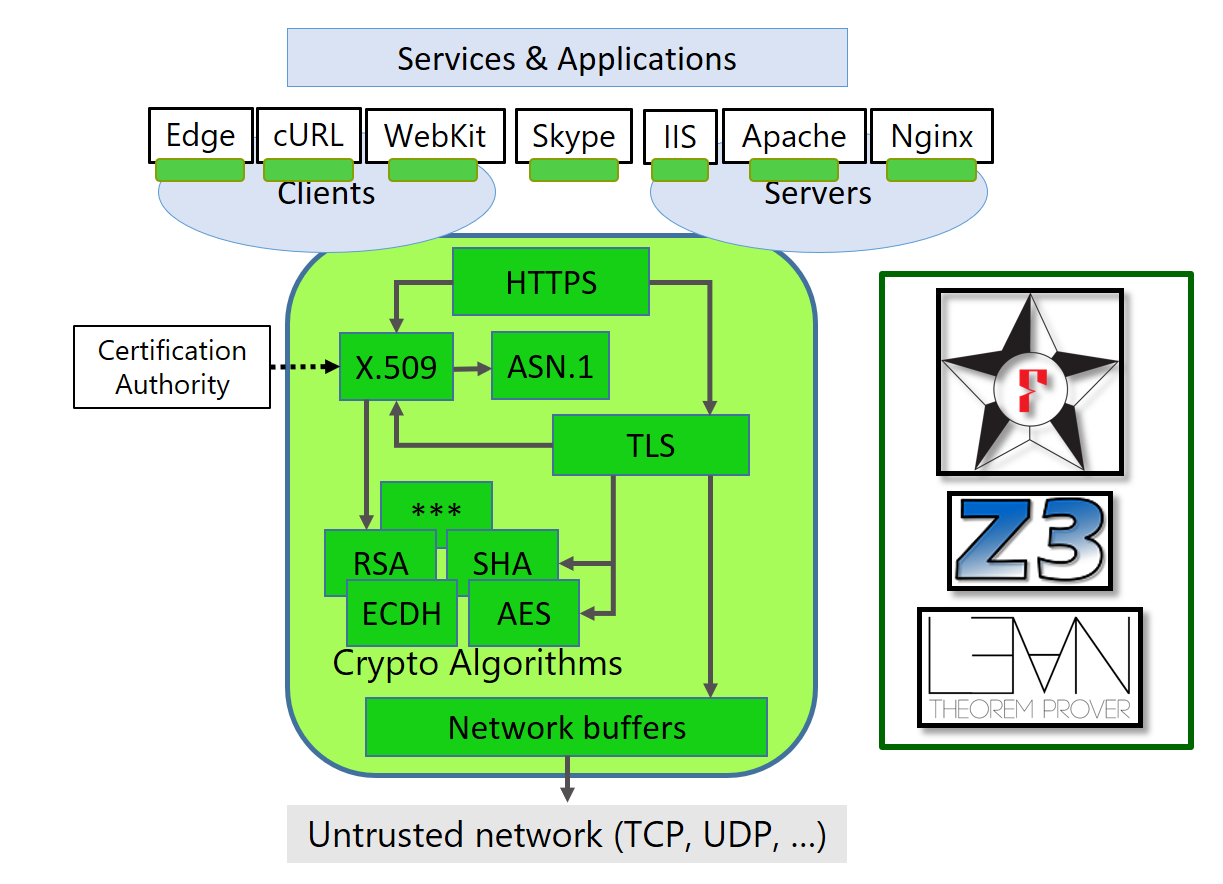
\includegraphics[scale=0.132]{SecureHTTPS.eps}
%%   \end{center}
%% \end{slide}

\begin{slide}
  \title{F*}
   Here is the factorial function in \Fstar:

\begin{alltt}
\textbf{val} fact: n:int\{n \(\geqslant\) 0\} \(\rightarrow\) Tot int

\textbf{let rec} fact n =
  \textbf{match} n \textbf{with}
    0 \(\rightarrow\) 1
  | \_ \(\rightarrow\) n * fact (n-1)
\end{alltt}

The annotation \texttt{n:int\{n \(\geqslant\) 0\} \(\rightarrow\) Tot
  int} is requesting the \Fstar compiler to prove that the factorial
function terminates (\texttt{Tot}) and returns a positive integer
(\texttt{\{n \(\geqslant\) 0\}}) when given as input a positive
integer.

\end{slide}

\begin{slide}
  \title{F*}

  \begin{itemize}

    \item \Fstar proves the function terminates using
      \textbf{well-founded recursion}.

    \item If the positivity constraint in the input \texttt{n:int\{n
      \(\geqslant\) 0\}} is removed, the typechecker of \Fstar informs
      that it cannot prove the property.

    \item Indeed, if \(n < 0\), the function does not terminate and a
      stack overflow occurs.

  \end{itemize}

\end{slide}

\begin{slide}
  \title{The Intel Pentium bug}

  \begin{center}
    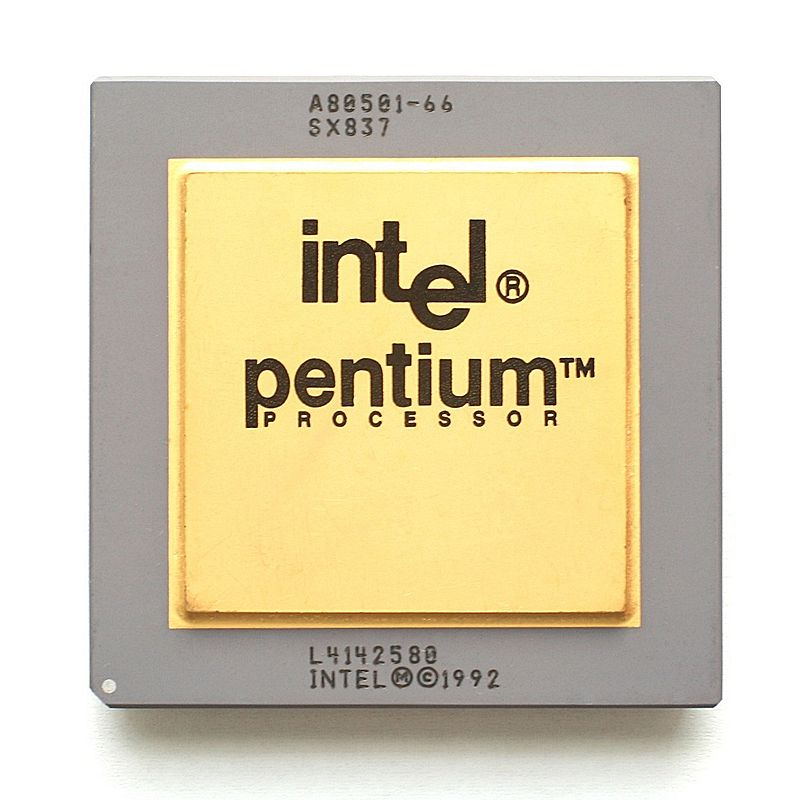
\includegraphics[scale=0.2]{Intel_Pentium_A80501.eps}
  \end{center}

  \centerline{CPU Intel Pentium, 66 MHz. Credit: Konstantin Lanzet, CC
    BY-SA 3.0}
\end{slide}

\begin{slide}
  \title{The Intel Pentium bug}

  \begin{itemize}

    \item The floating-point unit (FPU) of some Pentium processors
      (Intel) contained an error when a certain kind of division was
      performed.

    \item The FPU is a numeric coprocessor, to which the main
      processor (CPU) delegates computations for a speed up (about
      10$\times$).

    \item The error was discovered in 1994 by Thomas Nicely, a
      professor of mathematics at Lynchburg College (USA), who was
      performing number theoretic calculations.

    \item The division \emph{``\(1/824633702441.0\) is calculated
      incorrectly (all digits beyond the eighth significant digit are
      in error).'' -- Thomas Nicely.}

    \item Intel had to recall all faulty units, incurring a large
      cost, but also a very bad press (CNN) in what was at the time a
      competitive market.

  \end{itemize}

\end{slide}

\begin{slide}
  \title{The Intel Pentium bug}

  \begin{itemize}

    \item That bug is known as the ``Intel Pentium FDIV bug'', after
      the instruction for floating-point division.

    \item Intel reacted by investing in formal methods for the design
      of its chips.

    \item For example, John Harrison (Intel) has formally verified the
      correctness (of rounding) of various floating\hyp{}point
      algorithms using the \textbf{HOL Light prover} (a cousin of
      \Coq, also written in \OCaml).

    \item Also, various mathematical theorems in elementary number
      theory and real analysis were proved within the same framework.

    \item Intel combined theorem proving with a more automated
      approach when the state space is finite and small enough:
      \textbf{model checking}.

  \end{itemize}

\end{slide}

\begin{slide}
  \title{Model checking}

  \begin{itemize}

     \item \textbf{Model checking} was invented in the 80s to check
       the properties of concurrent systems.  (Clarke, Emerson, and
       Sifakis shared the 2007 Turing Award for their work.)

     \item Model checking reasons on the \textbf{states of a program}.

     \item It requires a way to define
       \begin{itemize}

         \item all possible states of a program, including those that
           should not be reached, and

         \item the execution of a program as the \textbf{transition}
           from one state to another (\textbf{traces}).

       \end{itemize}

     \item There is usually a very large, but \textbf{finite number of
       states}.

  \end{itemize}

\end{slide}


\begin{slide}
  \title{Model checking}

  \begin{itemize}

     \item \textbf{Temporal logic} is used to express properties of
       states

       \begin{itemize}

         \item \textbf{Safety}: a given (``bad'') state can never be
           reached;

         \item \textbf{Liveness}: a given (``good'') state will
           eventually be reached;

         \item \textbf{Reachability}: a given (``good'') state can be
           reached.

       \end{itemize}

     \item States and sets of states are usually defined with
       \textbf{logical formulas}.

     \item \textbf{SMT solvers} are often used to find a trace that
       leads to an undesirable state or prove the state is unreachable
       by exhausting all traces.

  \end{itemize}

\end{slide}

\begin{slide}
  \title{The takeaway}

  {\large What have you learnt in this lecture?}

\end{slide}

\begin{slide}
  \title{The takeaway}

  \begin{itemize}

    \item Bugs are everywhere and can be very costly.

    \item The \textbf{B method} helps manually narrowing the gap
      between specification and concrete implementation.

    \item \textbf{Abstract interpretation} runs an approximation of a
      program on an approximation of all possible inputs.

    \item Astrée, PolySpace and Frama-C are abstract interpreters
      written in \OCaml, used in the aerospace industry.

    \item \Coq is a \textbf{proof assistant} used to check
      mathematical theorems.

    \item \Coq is also used to write \textbf{certified compilers}.

  \end{itemize}

\end{slide}

\begin{slide}
  \title{The takeaway}

  \begin{itemize}

    \item \Fstar enables proving properties of functions using
      \textbf{type annotations}.

    \item \Fstar automatically proves the termination of recursive
      functions using \textbf{well-founded recursion}, but does not
      always succeed.

    \item \Fstar has been used to write efficient certified
      cryptographic libraries.

    \item \textbf{Model checking} is a technique to analyse all
      possible states of a program and prove that some (bad) states
      are unreacheable.

    \item States and sets of states are defined with \textbf{logical
      formulas}.

    \item \textbf{SMT solvers} are used to find a trace reaching
      undesired states, or prove the absence of such a trace.

%    \item CubicleW is a model checker written in OCaml, used by Intel
%      to check processor pipeline reordering

  \end{itemize}

\end{slide}

\end{document}
